% ============================================================
%  深圳大学实验报告模板(SZU Experiment Report Template)
% This template can be modified according to the specific requirements of your experiment or project.
% Produced by: Chao Fan and Kewei Ou, AI School of SZU
% ============================================================

\documentclass[a4paper,12pt]{article}

% ----------------------------
% 中文与字体支持
% ----------------------------
\usepackage{fontspec}    % 字体支持
\usepackage{xeCJK}       % 中文字体支持
\setCJKmainfont{Noto Serif CJK SC} % 设置中文字体(Overleaf自带Noto字体)

% ----------------------------
% 页面设置与常用宏包
% ----------------------------
\usepackage{geometry}    % 页面边距控制
\geometry{left=1in, right=1in, top=1in, bottom=1in}

\usepackage{longtable}   % 支持长表格
\usepackage{graphicx}    % 插入图片
\usepackage{fancyhdr}    % 页眉页脚控制
\usepackage{tikz}        % 绘制框线等图形
\usetikzlibrary{calc}    % 坐标计算
\usepackage{verbatim}    % 显示代码块
\usepackage{float}       % 控制图片浮动位置([H]参数)

% ----------------------------
% 页眉页脚设置
% ----------------------------
\pagestyle{fancy}
\fancyhf{} % 清空默认页眉页脚
\fancyhead[L]{深圳大学实验报告} % 左侧页眉文字
\fancyhead[C]{} % 中间空
\fancyhead[R]{} % 右侧空

% ============================================================
%                      文档开始
% ============================================================

\begin{document}

% ============================================================
% 封面页
% ============================================================
\begin{titlepage}
    \centering
    \vspace*{2cm}
    {\Huge \textbf{深 \quad 圳 \quad 大 \quad 学 \quad 实 \quad 验 \quad 报 \quad 告}}\\[2cm]

    {\Large 课程名称:\underline{\hspace{2.5cm}Python程序设计\hspace{2.5cm}}}\\[0.8cm]
    {\Large 项目名称:\underline{\hspace{3.4cm}外星人入侵\hspace{3cm}}}\\[0.8cm]
    {\Large 学\quad\quad 院:\underline{\hspace{2.8cm}人工智能学院\hspace{3cm}}}\\[0.8cm]
    {\Large 专\quad\quad 业:\underline{计算机科学与技术(IEEE荣誉班)}}\\[0.8cm]
    {\Large 指导教师:\underline{\hspace{4cm}樊超\hspace{4cm}}}\\[0.8cm]
    {\Large 报 告 人:\underline{\hspace{0.5cm}陈泓佳\hspace{0.5cm}}
        \quad 学号:\underline{\hspace{1cm}2024104023\hspace{0.5cm}}}\\[0.8cm]
    {\Large 实验时间:\underline{\hspace{2cm}2025年11月19日\hspace{2cm}}}\\[0.8cm]
    {\Large 提交时间:\underline{\hspace{2cm}2025年11月20日\hspace{2cm}}}\\[2cm]

    \vfill
    {\Large 教务处制}
\end{titlepage}

\newpage

% ============================================================
% 正文部分
% ============================================================
% Figure
\begin{figure}[t]
    \centering
    \includegraphics[width=0.92\linewidth]{figs/image.png}
    \caption{文件中类的成员方法供给关系图}
    \label{fig:vit-arch}
\end{figure}
% Oringin Objectives
\section{原书内容复现}
\indent 该项目原有 8 个 Python 文件,我在修改后共包含 9 个文件。如图所示,上图箭头文件1指向文件2表示文件1向文件2提供了对象并任由其查看与修改。体现了面向对象程序设计思想\\
\indent alien\_invasion.py 是主程序,通过调用其他类的属性与方法控制游戏流程。例如在 \_check\_keydown\_events 中修改 Ship 对象的 moving\_right 等属性来实现飞船移动。\\
\indent Settings 类 负责管理所有游戏参数(飞船、子弹、外星人速度等)。该类实例在主程序中创建,其它类通过传入 AlienInvasion 实例来访问全局设置。ScoreBoard 类 用于管理界面文字,包括字体、颜色、位置和动态更新的分数等显示内容。GameState 类 用于记录与重置游戏状态。\\
\indent Ship 类 定义飞船的大部分属性(位置、图像、移动方式等),并实现移动检测、边界判断、位置重置与绘制等方法。Alien 类 与 Ship 类结构类似,每个 Alien 实例代表一个独立外星人对象。\\
\indent Button 类 则负责“Play”按钮的外观与绘制,点击逻辑在主程序中处理。Bullet 类 定义子弹的矩形外形、初始位置以及移动与绘制方法,子弹与外星人的碰撞检测逻辑同样写在主程序中。外星人与子弹均以 Group 的形式统一管理。
% Experiment Objective
\section{实验内容的实现}
\indent 实验要求我们在原书的基础上实现以下两个功能:
\begin{enumerate}
    \item[功能1]: 实现最高分记录;\\
    原书已提供最高分变量和GameState中的 high\_score 属性,其值在游戏运行中不会消失,只会在退出游戏时重置。因此,只需在退出前将最高分写入同目录下的txt文件,并在下次启动时读取即可。
    我在 AlienInvasion 类中新增了store\_high\_score 方法,并在用户按下 q 退出时调用。GameState 的初始化改为接收外部传入的 high\_score,而非默认 0。同时在 AlienInvasion 的初始化中尝试读取 txt 文件内容,若不存在文件则将 high\_score 设为 0。
    \item[功能2]: 实现外星人会发射子弹且我方飞船可拥有护盾;\\
    我创建了一个外星人子弹类,内部与飞船子弹类差不多,颜色和发射方向不同,以及初始位置在外星人的midbottom处。一开始我在想要把子弹当作一个全局Group装入AlienInvasion类里面统一管理,后面仔细想想觉得不妥,万一以后要造多元化的外星人修改起来就很麻烦了,于是乎,我让每一个外星人都装有一个外星人子弹的Group,并设置Settings类中有个shoot\_tr属性来控制发射频率,创建一个时钟来检测是否到达可发射时间,Alien类中多一个记录上次发射的时间(与当前时间差值达到tr便可发射),这样每次要刷新的时候只要遍历一遍外星人(外星人不多),挨个刷新其Group就完事了,与飞船collision的实现也同理,遍历检查。至于护盾实现,由于时间有限,我并没有将其具象化,而是抽象成了一个判断:首先在Ship上面设置一个shield的bool值,1表示开,0表示关;其次将开关信息存入ScoreBoard类内并实时刷新放置在屏幕上提醒用户;最后在collision的那部分做一个bool判断,护盾没开就ship\_hit,护盾开了就设置bool值为0,当然还有重启时的初始化1,不再赘述。
\end{enumerate}

% Implementation Details
\section{个人创新的实现}
思来想去,游戏做到这里的可玩性还是太低了,要想别人玩你的游戏玩得high,还得再做点调整。
\begin{enumerate}
    \item[Part 1]: Random is all you need;\\
    单机游戏之所以能够经久不衰,除了靠剧情,靠的也就只有每次用户打开时的惊喜感(随机性)。因此,我把外星人的速度以及发射子弹的频率取消,改成输入了两段段区间,而外星人在获取速度和shoot\_tr的时候也不再是简单地从Settings中获取,而是在Settings中设置好的范围内分别随机取数。这样一来,你每次打开游戏时候的场景都不一样,有些外星人快如闪电,有些外星人慢如蜗牛,有些外星人拿了加特林,有些外星人拿了小水枪。运气好这局很简单,运气不好这局连大神都救不了,大大提高了可玩性。
    \item[Part 2]: 加强护盾的功能;\\
    实验过程中我发现,经过上面一改,外星人子弹如春雨般不断地下,护盾的作用聊胜于无,游戏难度太大使人退游。于是我想出一计,我在用户输入部分多加了一个shift,一旦你按下shift,被击碎的护盾就可以恢复。是不是太简单了?并非如此。首先外星人在不断逼近,你不可能一直按shift(还会触发粘滞键);并且我取消了护盾损坏的提示,用户唯一获取护盾是否开启的方法,只能自己注意看左上角的护盾信息;再者,外星人的子弹数量(默认)真挺多的,有时候就算你有反应过来要及时打开护盾,也来不及按下。\\
\end{enumerate} 
以上,游戏开发正式完成。
\section{实验收尾与个人反思}
实验代码与本篇实验报告的代码均会在GitHub上面发布,欢迎老师来看。地址:https://github.com/ZSZH12138/Homework-of-Python.git\\
两个存有代码的文件夹里面分别有两个README文件。\\
本次实验我学习到了如何从零使用Python开发一款属于自己的游戏,多使用了面向对象的思想,大大提升了我的编码能力。虽然过程艰辛,但是结果还是好的,希望以后能有机会接触到更多有意思的代码编写项目。
\newpage

% ============================================================
% 批阅与成绩评定页
% ============================================================

% 绘制正文外框(包含批阅区域)
\begin{tikzpicture}[remember picture, overlay]
  \draw[thick] 
    ($(current page.north west)+(2cm,-3cm)$) 
    rectangle 
    ($(current page.south east)+(-2cm,2.5cm)$);
\end{tikzpicture}

\vspace{1cm}

% 批阅区
\noindent \textbf{指导教师批阅意见:}
\vspace{5cm}
\hfill

\vspace{1cm}

\noindent \textbf{成绩评定:}
\vspace{2cm}
\hfill

\vspace{1cm}

\noindent \textbf{指导教师签字:}
\vspace{2cm}
\hfill

\vspace{1cm}

% 备注部分
\noindent \textbf{备注:}
\begin{itemize}
    \item 报告内的项目或内容设置,可根据实际情况加以调整和补充。
    \item 教师批改学生实验报告时间应在学生提交实验报告时间后 10 日内。
\end{itemize}

% ============================================================
%                      文档结束
% ============================================================

\end{document}

